\documentclass{article}
\usepackage{fancyhdr}
\usepackage{titlesec}
\usepackage{graphicx}
\graphicspath{ {./img/} }
\usepackage{multirow}
\usepackage{hyperref}
\usepackage{blindtext}
\hypersetup{
    colorlinks=true,
    linkcolor=blue,
    filecolor=magenta,      
    urlcolor=blue,
}
% \usepackage[a4paper, portrait, margin=1in]{geometry}

\pagestyle{fancy}
\fancyhf{}
\lhead{Modul 0 Praktikum Game Development}
\rfoot{\footnotesize Page \thepage}
\lfoot{\footnotesize Mahyus Ihsan, S.Si, M.Si \newline Jurusan Informatika Universitas Syiah Kuala \newline Modul oleh : Diky Wahyudi, Rendika Rahmaturrizki}
\renewcommand{\headrulewidth}{1pt}
\renewcommand{\footrulewidth}{1pt}

\titleformat*{\section}{\small\bfseries}

\begin{document}
    \begin{center}
        \textbf{Modul 0 Praktikum Jaringan Komputer}

        \textbf{Membuat Akun Unity dan Instalasi Unity}
    \end{center}

    \section*{Deskripsi Singkat}
    Dalam modul ini, Anda akan mempelajari langkah-langkah dasar untuk memulai pengembangan game menggunakan Unity. Setelah memiliki akun, langkah berikutnya adalah mengunduh dan menginstal UnityHub. Setelah UnityHub terinstal, lalu anda dapat mengunduh versi Unity yang diinginkan. Pada modul ini, Anda akan mempelajari langkah-langkah untuk membuat akun Unity dan menginstal UnityHub.

    \section*{Tujuan}
    \begin{enumerate}
        \item Memahami cara membuat akun Unity
        \item Memahami cara menginstal UnityHub
        \item Memahami cara mengunduh versi Unity
    \end{enumerate}

    \begin{flushleft}
        \textbf{Materi 1 - Membuat Akun Unity}
        \newline

        Pada materi ini, Anda akan mempelajari cara membuat akun Unity. Langkah-langkahnya adalah sebagai berikut:

        \begin{enumerate}
            \item Buka browser dan akses situs web Unity di alamat \href{https://unity.com/download}{https://unity.com/download}
            
            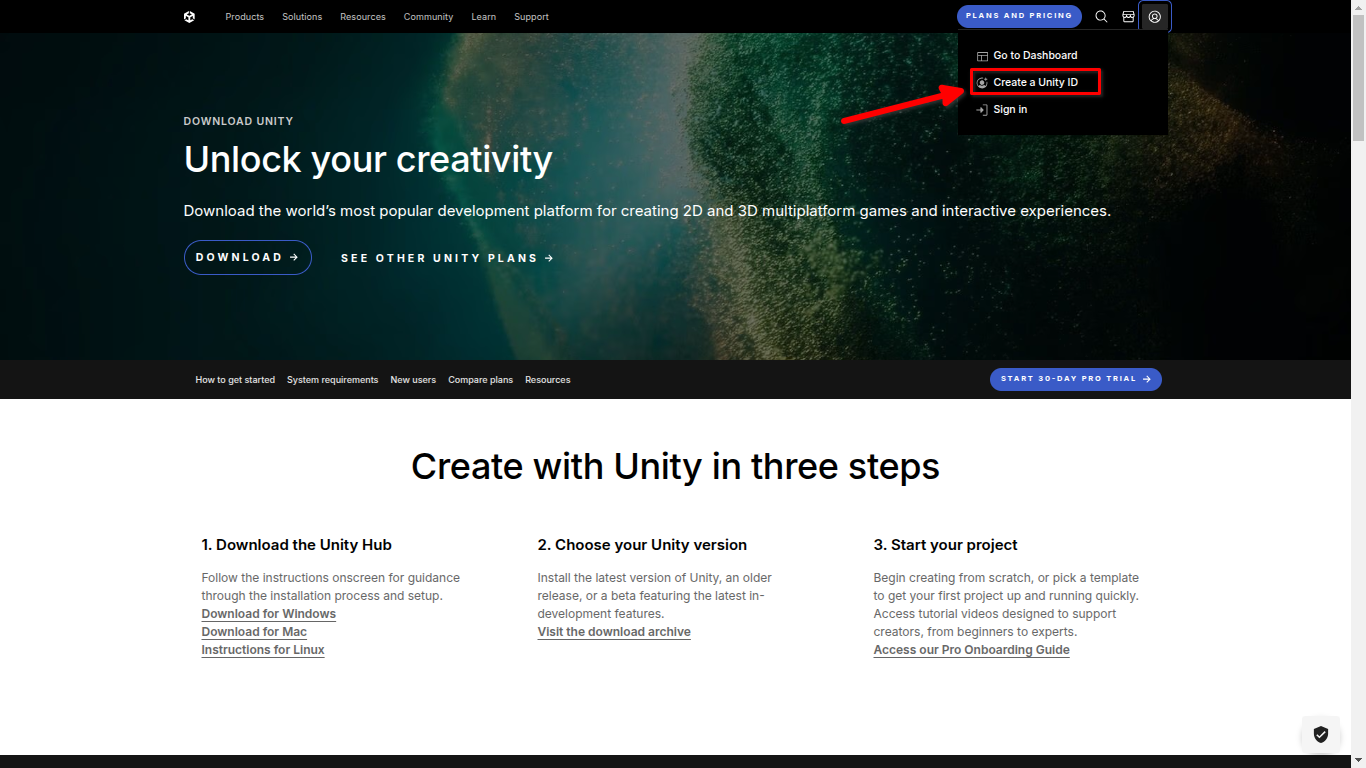
\includegraphics[scale=0.3]{01_singup_menu.png}

            \item Klik tombol \textit{Sign In} di pojok kanan atas halaman.
            \item Klik tombol \textit{Create a Unity ID}.
            \item Isi formulir pendaftaran dengan informasi yang benar.

            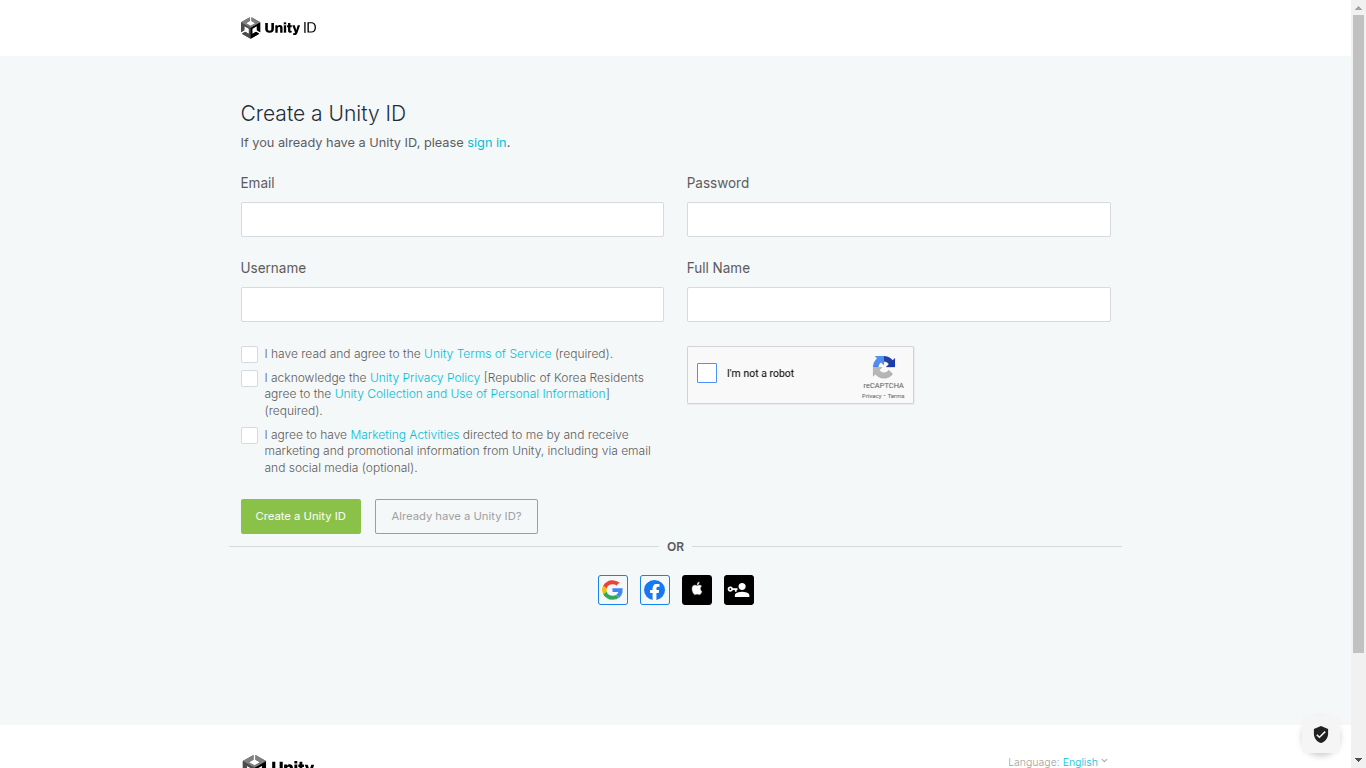
\includegraphics[scale=0.3]{02_create_account.png}

            \item Klik tombol \textit{Create Unity ID}.
            \item Buka email yang digunakan untuk mendaftar dan klik tautan verifikasi yang dikirim oleh Unity.
            \item Setelah verifikasi berhasil, Anda dapat masuk ke akun Unity Anda.
        \end{enumerate}
    \end{flushleft}

    \begin{flushleft}
        \textbf{Materi 2 - Instalasi UnityHub}
        \newline

        Pada materi ini, Anda akan mempelajari cara menginstal UnityHub. Langkah-langkahnya adalah sebagai berikut:

        \begin{enumerate}
            \item Buka browser dan akses situs web Unity di alamat \href{https://unity.com/download}{https://unity.com/download}

            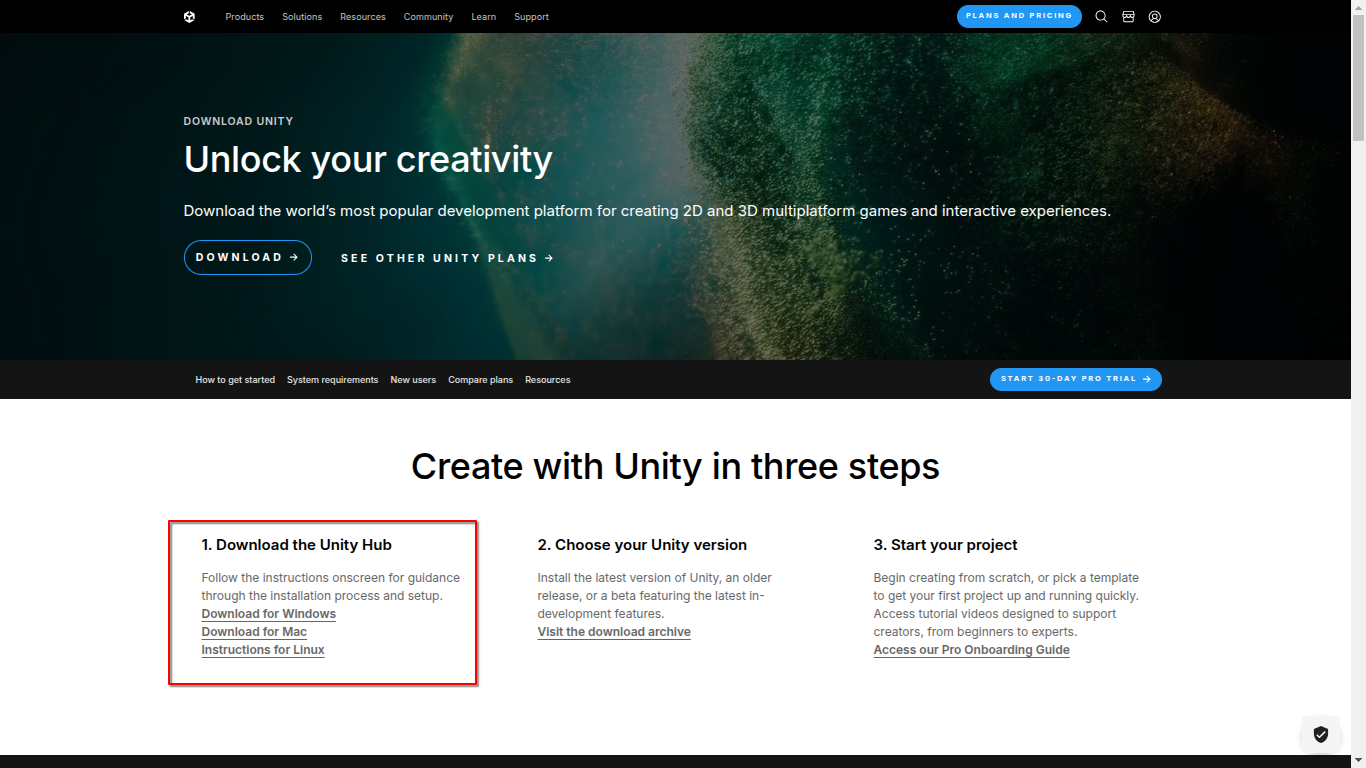
\includegraphics[scale=0.3]{03_download_unity.png}

            \item Pada menu \textit{Download Unity Hub} pilih menu sesuai dengan sistem operasi anda.
            \item Buka file yang telah diunduh dan ikuti petunjuk instalasi.
            
            \begin{center}
                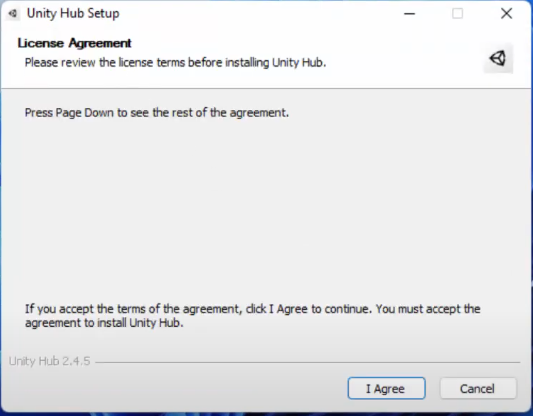
\includegraphics[scale=0.5]{04_install_unity_1.png}
                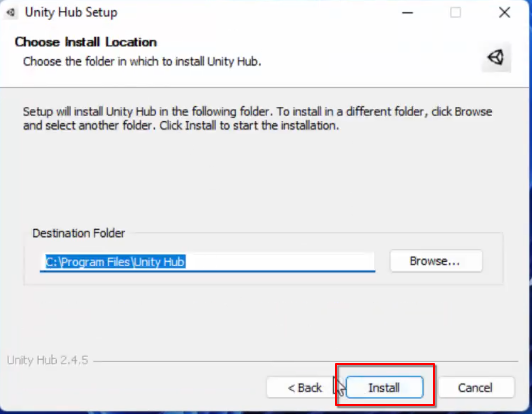
\includegraphics[scale=0.5]{05_install_unity_2.png}
            \end{center}

            \item Setelah instalasi selesai, buka UnityHub dan login dengan akun Unity yang telah dibuat sebelumnya.
            
            \begin{center}
                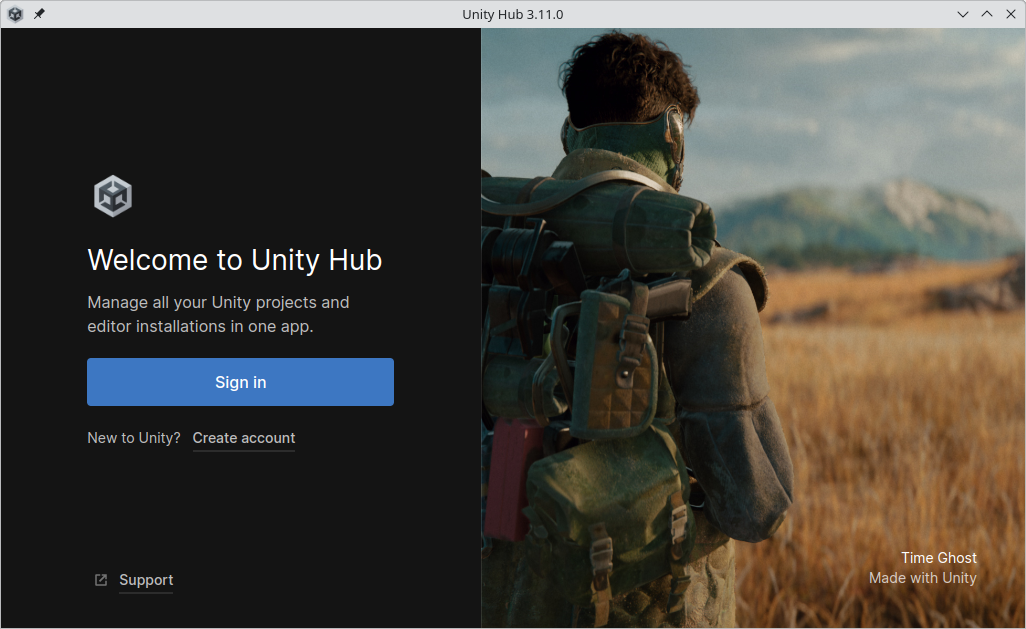
\includegraphics[scale=0.3]{06_unity_login.png}
            \end{center}
            \item Lakukan instalasi UnityEditor sesuai dengan versi yang diinginkan (Pada praktikum ini akan digunakan Unity 6).
            
            \begin{center}
                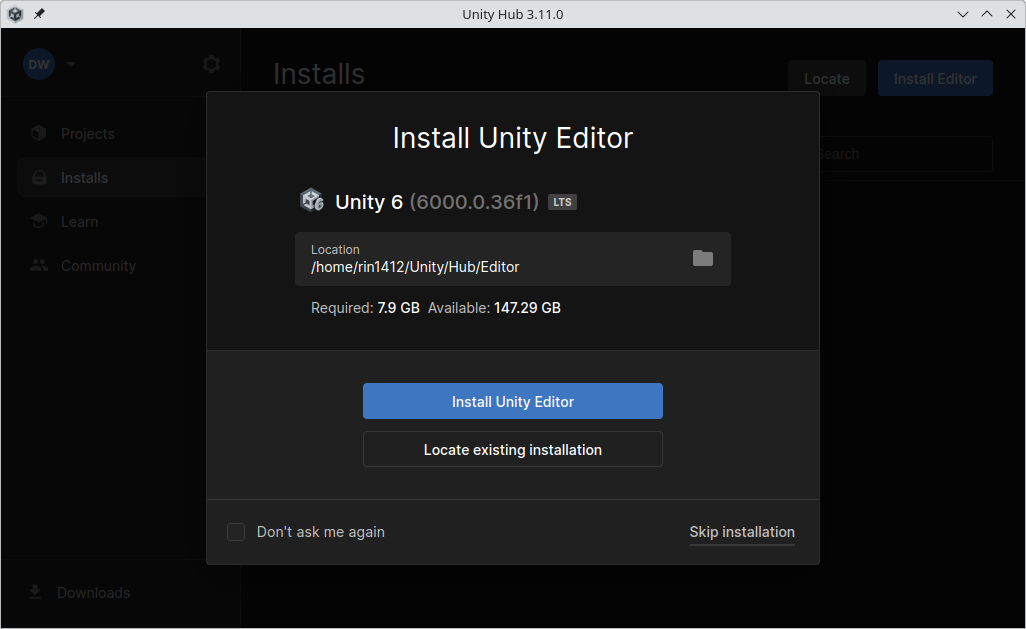
\includegraphics[scale=0.3]{07_unity_editor.png}
            \end{center}
            \textbf{Note: Pastikan Anda memiliki koneksi internet yang stabil karena proses ini membutuhkan unduhan data yang cukup besar.}

            \item Tunggu hingga proses download selesai.
            \begin{center}
                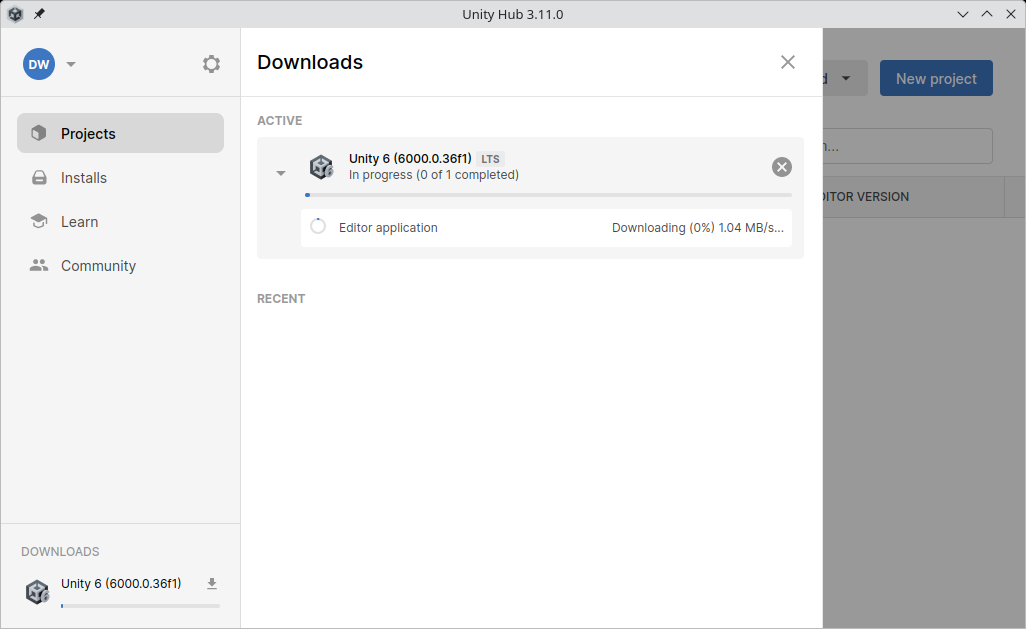
\includegraphics[scale=0.3]{08_download.png}
            \end{center}

            \item Setelah proses download selesai, Anda dapat membuka Unity Editor dan mulai membuat game.
            
            \begin{center}
                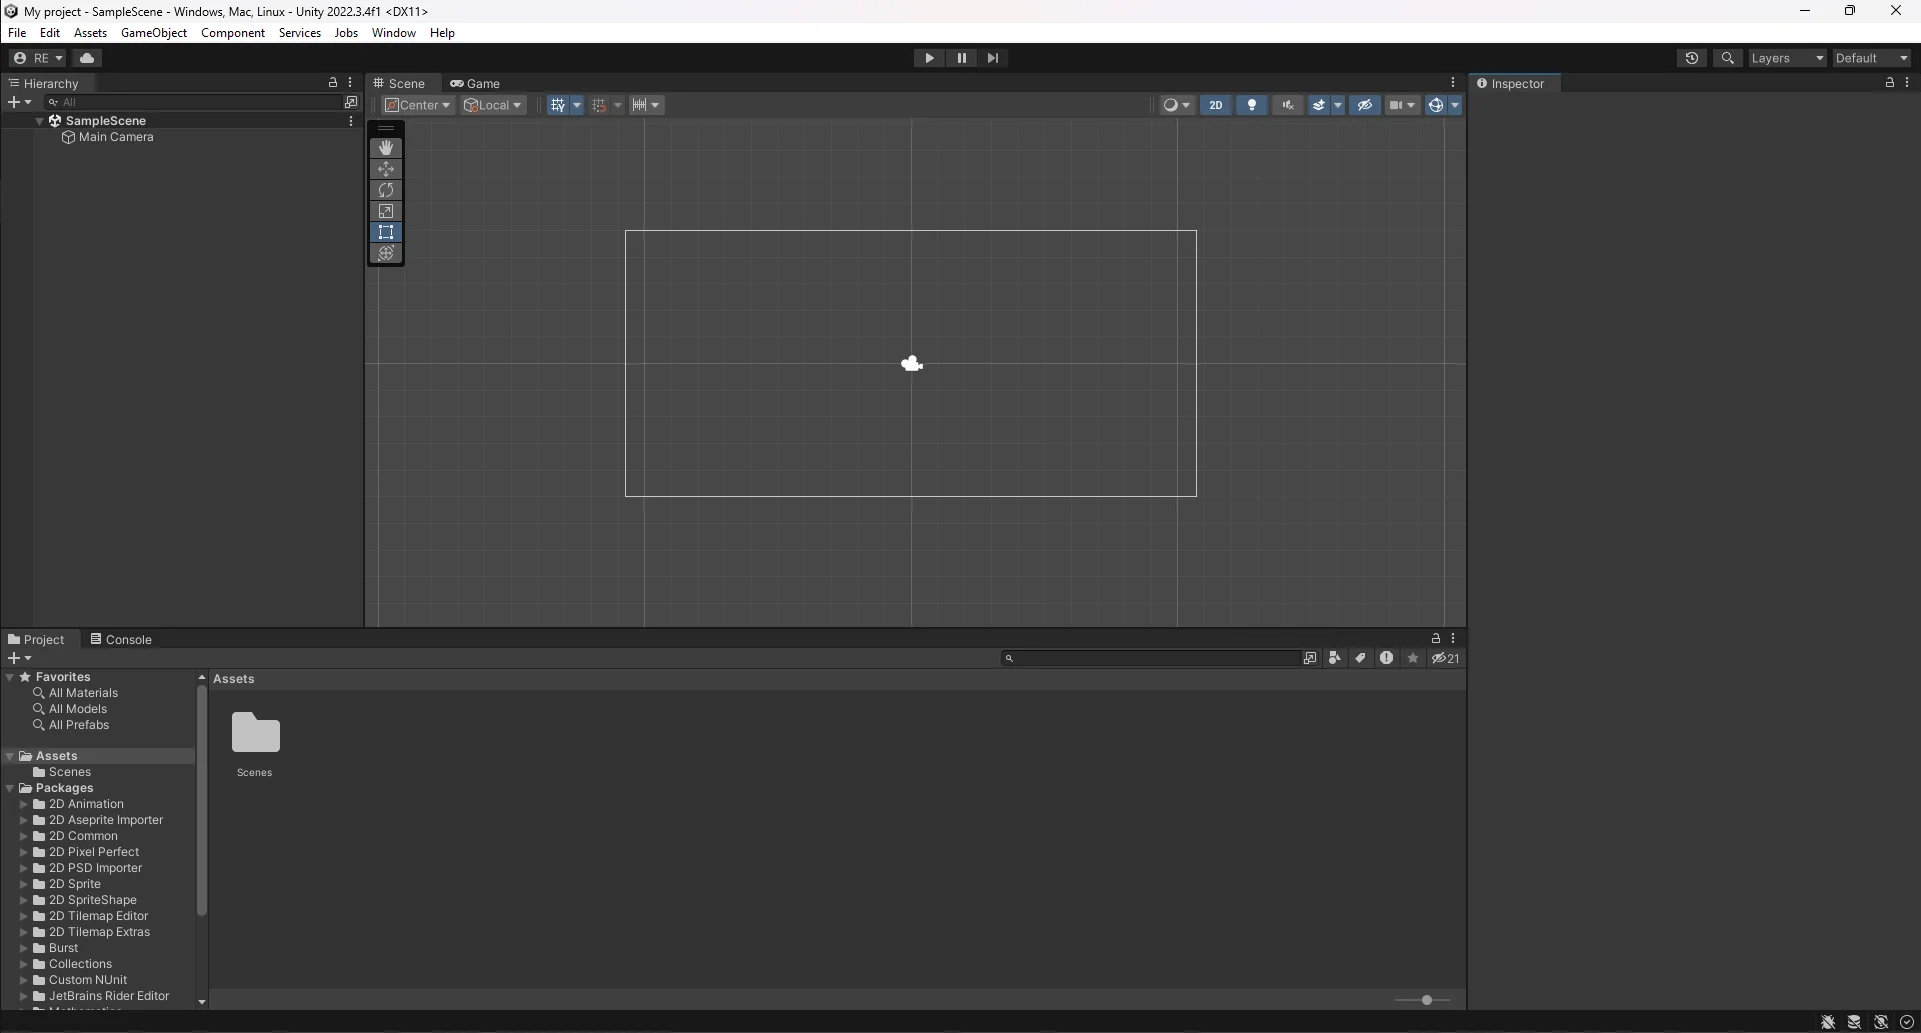
\includegraphics[scale=0.11]{09_editor.png}
            \end{center}
        \end{enumerate}
    \end{flushleft}

    \newpage
    \begin{flushleft}
        \textbf{Tugas}
        \newline

        \begin{enumerate}
            \item Kerjakan seluruh langkah pada Materi 1 dan Materi 2.
        \end{enumerate}
    \end{flushleft}
\end{document}